\documentclass[a4paper,fleqn,12pt]{article}

%%%%%%%%%%%%%%%%%%%%

\input{../common/common.tex}
%%%%%%%%%%%%%%%%%%%%%%%%%%%%%%%%%%%%%%%%%%%%%%%%%%%%%%%%%%%%%%%%%%%%%%%%%%%%%%%
%% Project-specific configuration
%%%%%%%%%%%%%%%%%%%%%%%%%%%%%%%%%%%%%%%%%%%%%%%%%%%%%%%%%%%%%%%%%%%%%%%%%%%%%%%

\author{Joey Harrison}
\title{Programmable I/O for Flexible Interfaces in Embedded RISC-V Systems}
%\supervisor{Your supervisor's name}
% \yearofstudy{3\textsuperscript{rd}}

%%%%%%%%%%%%%%%%%%%%%%%%%%%%%%%%%%%%%%%%%%%%%%%%%%%%%%%%%%%%%%%%%%%%%%%%%%%%%%%


\assignment{Project specification}

%%%%%%%%%%%%%%%%%%%%

\pagestyle{plain}
\renewcommand{\headrulewidth}{0.0pt}

\makeatletter
\fancypagestyle{plain}{
	\fancyhf{}
    \fancyfoot[C]{\thepage}
}
\makeatother

%%%%%%%%%%%%%%%%%%%%
\begin{document}

\input{../common/titlepage.tex}

\pagestyle{plain}

\section{Introduction}
Traditionally, general-purpose microcontrollers necessitate the inclusion of a wide variety of hardware interfaces such as UART, SPI, and I2C to interface with a broad range of peripherals. Each of these interfaces has different hardware requirements, and is costly in development time, chip area, and system power. These interfaces are often emulated over general-purpose I/O interfaces using software techniques, but such techniques are usually inefficient and have poor performance.

The aim of this project is to develop state machine-based programmable I/O blocks which are able to emulate any hardware interface or implement any communication protocol, via programming using a small assembly-like DSL. These blocks will then be integrated with open-source RISC-V cores to create a flexible and compact microcontroller, ideal for use in low power, low cost embedded applications. This microcontroller would be applicable for any use in which traditional hardware interfaces are needed, but also for applications which have specific or highly custom I/O requirements, without the need for programmable logic (as is found in FPGAs) or custom hardware.

\section{Background}

The primary purpose of embedded systems and microcontrollers is usually to interact with the real world via sensors, actuators, LEDs, speakers, etc, but communicating with such hardware can be difficult due to the need for high frequencies and precise timing requirements. Computers and microcontrollers include dedicated hardware for high-speed interfaces: SATA and PCIe are common in desktop-class hardware and used to interface with consumer hardware, but interfaces such as UART, SPI, I2C, PWM and I2S are more general-purpose buses usually found in microcontrollers and designed for use with a wide variety of electronics devices. These protocols are also simpler and cheaper (in terms of power, space and money) to implement than the likes of SATA, making them ideal for lower-cost microcontrollers. All of these interfaces have different hardware and software requirements, and the cost and complexity associated with implementing all of these in a device may mean you end up with lots of interfaces you don't need, or not enough of a single type of interface.

A common alternative to using dedicated hardware is to use the CPU to control GPIO (General Purpose I/O) pins, implementing the control and timing processes in software: a process known as 'bit-banging'. However, general-purpose software processors are generally not designed to do this, and maintaining precise timing requirements at high speed is very hard, especially when the processor has other work to do. For example, SPI can run at up 100MHz, a speed which is impossible to maintain on most consumer microcontrollers, especially lower-power ones \cite{picosdk}.

The usual solution to custom interface requirements is FPGAs (Field Programmable Gate Arrays): programmable hardware devices that can be configured by an engineer to implement whatever hardware they wish. These are very flexible but come at a high price, and there is also still the need for software processor alongside it. 'Soft' CPU cores can be implemented in FPGAs alongside other hardware devices, and some embedded systems such as the Xilinx Zynq SoCs combine traditional ARM processing cores with programmable logic slices, connected over various buses \cite{zynq}. FPGAs also present a very different programming model, as programmers are not writing software but designing hardware.


\begin{figure}[b!]
    \centering
    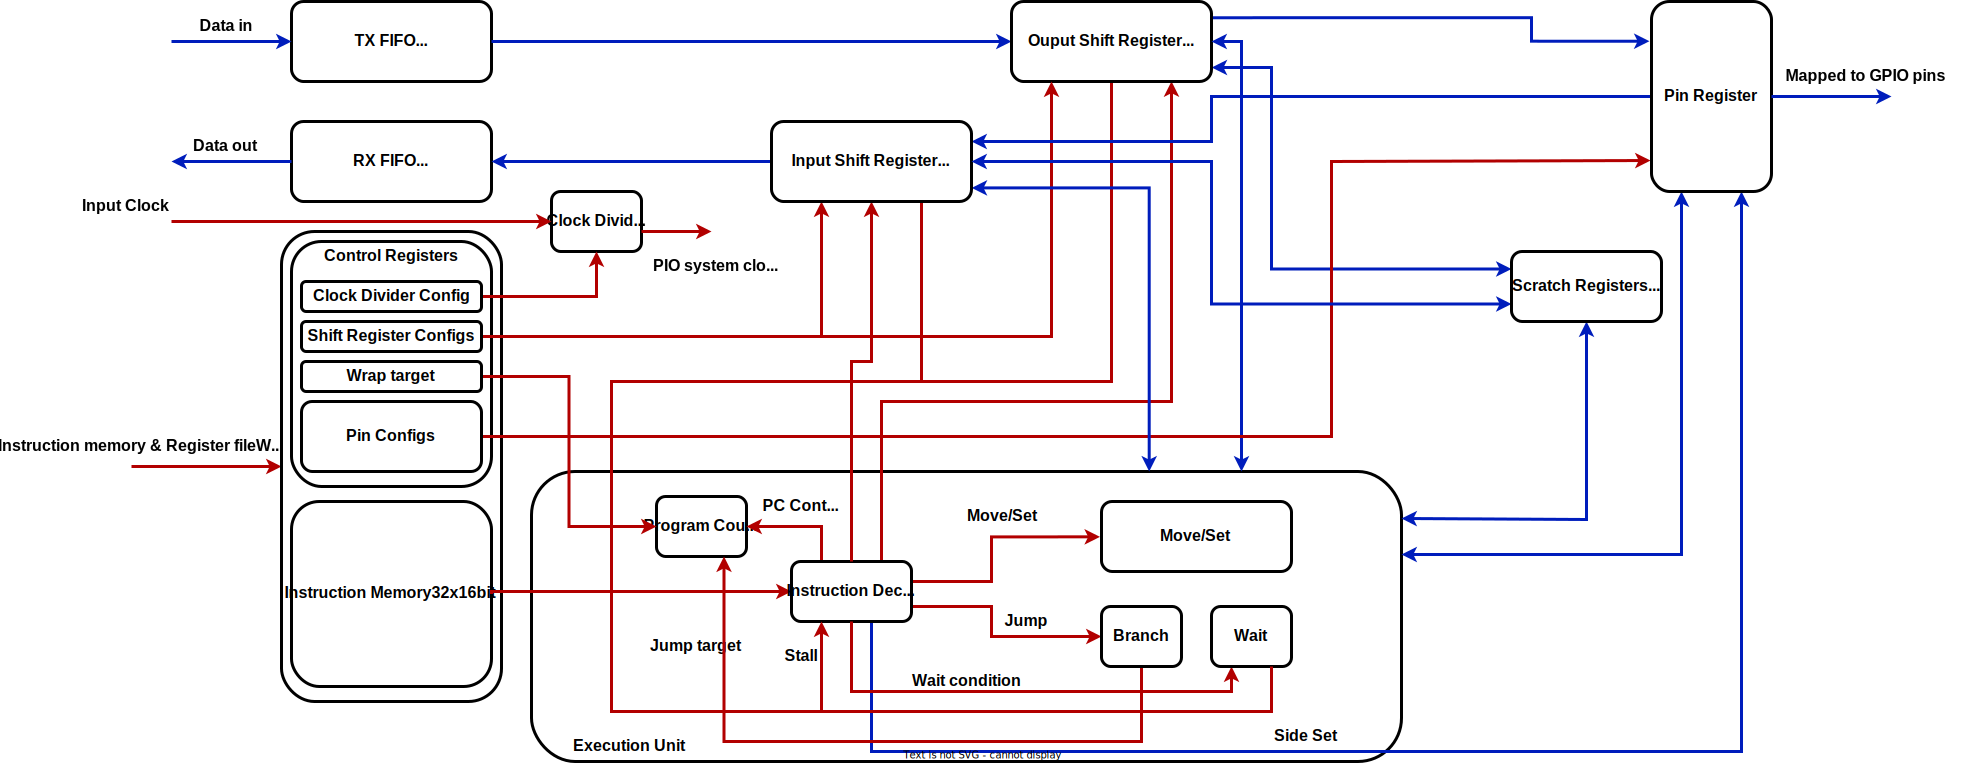
\includegraphics[width=0.7\textwidth]{../img/pio-block.jpg}
    \caption{A PIO block from the RP2040 \cite{rp2040}}
    \label{fig:pio-block}
\end{figure}


It is this problem that we intend to tackle: developing a flexible, low cost, easy to use hardware interface for embedded systems. The inspiration for this comes from the RP2040: a dual-core ARM-based microcontroller designed by Raspberry Pi Ltd released in 2021. The flagship feature of the RP2040 is PIO (Programmable I/O blocks), which are as I have described in my introduction. Two PIO blocks are included in the RP2040, each of which includes 4 state machines, as shown in figure \ref{fig:pio-block}.




The PIO state machines are designed specifically for I/O, able to move data with the speed and timing precision required for high-speed serial I/O interfaces such as SPI, UART and even VGA/DPI. As shown in figure \ref{fig:pio-sm}, each state machine consists of:

\begin{itemize}
    \item Two 32-bit shift registers
    \item Two 32-but scratch registers
    \item A fractional clock divider
    \item Flexible GPIO pin mapping
    \item 4x32 bit Rx/Tx FIFOs connected to the system bus, able to sustain up to one word per clock to/from DMA
\end{itemize}

\begin{figure}[H]
    \centering
    \includegraphics[width=0.7\textwidth]{../img/rp2040-state-machine.png}
    \caption{An overview of a PIO State Machine \cite{rp2040}}
    \label{fig:pio-sm}
\end{figure}

The state machines are programmed using \texttt{pioasm} (PIO Assembly). An example program is shown in listing \ref{pioasm} to output a simple square wave.

\begin{listing}[b]
    \vspace{0.5cm}
    \begin{minted}{asm}
    .program squarewave
    set pindirs, 1   ; Set pin to output
again:
    set pins, 1 [1]  ; Drive pin high then delay for one cycle
    set pins, 0      ; Drive pin low
    jmp again        ; Set PC to label `again`
    \end{minted}
    \caption{PIO Assembly to output a square wave \cite{rp2040}}
    \label{pioasm}
\end{listing}

Another similar hardware device from which we may draw inspiration is the Time Processor Unit (TPU), a device found in some Motorola microcontrollers. The TPU is a coprocessor engine designed to handle complex timing and I/O tasks, independently of the CPU. The TPU consists of a microengine and scheduler for precision timing and execution of instructions, and up to 16 timer channels connected to external pins. Communication with the rest of the system is done via a shared dual-port RAM. Similar to the RP2040, it works by processing and executing microinstructions written by the programmer. Figure \ref{fig:tpu} shows a high-level block diagram of the TPU \cite{tpu}.

\begin{figure}[]
    \centering
    \includegraphics[width=0.8\textwidth]{../img/tpu.jpg}
    \caption{An overview of a Time Processor Unit \cite{tpu}}
    \label{fig:tpu}
\end{figure}

Another major component of this project will be CHISEL, and rocket chip. intend to explore chisel as a HDL

\section{Objectives}
Our goal is to expand on the prior work of current hardware devices and use CHISEL and Rocket Chip to build open source programmable I/O devices, integrated with RISC-V cores to create a complete microcontroller. Implementation will target FPGAs, as this allows for rapid prototyping and easy implementation and testing of hardware. The functional and non-functional requirements for our I/O device are as follows:
\begin{itemize}
    \item The device should be implement in CHISEL (NF)
    \item The device should connect to external pins on the FPGA (F)
    \item The device should be able to receive input
\end{itemize}


- be implemented in chisel
- Proof of concept i/o chisel code
- Lay out high-level block design on paper
- Extend proof of concept into skeleton for in HDL
- Implement HDL one module at a time
- Unit test HDL in simulation

The secondary goal, once the HDL implementation is complete, is to build a microcontroller integrating the devices. The requirements for this are as follows:
\begin{itemize}
    \item
\end{itemize}

Possible extensions to the project, should time permite, include:
\begin{itemize}
    \item
\end{itemize}

\section{Timeline}

Table \ref{tab:timeline} gives a rough timeline for my project. Each of the tasks in the table is dependent upon the previous. There are a few notes of context for this:

\begin{itemize}
    \item Week 1 is the start of Term 1
    \item Week 15 is the start of Term 2
    \item The final report is due in Week 31
    \item I have planned to do more work in Term 2, as I am taking more modules in term 1 than term 2.
\end{itemize}


\begin{table}[h!]
    \centering
    \begin{tabular}{|c|l|}
        \hline
        \textbf{Week(s)} & \textbf{Task}                                                       \\ \hline
        1-2              & Background research                                                 \\ \hline
        3-5              & Implement proof of concept I/O device in CHISEL                     \\ \hline
        6-8              & Lay out high-level block design                                     \\ \hline
        8-11             & Extend proof of concept into project skeleton based on block design \\ \hline
        12-19            & Write HDL code, implementing and testing one module at a time       \\ \hline
        20               & Develop and run integration tests in simulation                     \\ \hline
        21-22            & Use Rocket Chip to integrate device with RISC-V cores               \\ \hline
        23-25            & Load microcontroller onto FPGA and run tests                        \\ \hline
        26-31            & Write report                                                        \\ \hline
    \end{tabular}
    \caption{Project Timeline}
    \label{tab:timeline}
\end{table}

\section{Methodology}
This project is very practical, and the bulk of my time will be spent writing and testing HDL code. As such, an appropriate software engineering methodology is required. My approach will be very plan based, first laying out a high-level block design on paper, then moving to lay out skeleton HDL code, then writing the code one module at a time. Any iteration on the design will require going back to the block design, necessitating a waterfall-style approach to development. When it comes to

When it comes to testing, I intend to utilised test-driven development (TDD) heavily. Functional verification of hardware is very important
testing methods (tdd)
\section{Resources}
\section{Risk Assessment}
\section{Legal, Social and Professional Issues}
\bibliographystyle{../common/plainnat}
\bibliography{../common/bibliography}

\end{document}
